%! Author = adnansiddiquei
%! Date = 04/06/2024

\section{Results}\label{sec:results}
To assess and demonstrate the performance of our AstroCLIP model, we reproduce a subset of the downstream tasks from
the original implementation.
The held-out validation set (composing of 39,599 of the 197,976 image-spectra pairs) was used to evaluate the performance
by assessing the accuracy of zero-shot k-NN redshift estimations and qualitative similarity retrieval tasks.
Notation used in this section intentionally follows that of the original paper for the reader's convenience.

\subsection{Zero-shot k-NN Redshift Estimation}\label{subsec:results-redshift-regression}
\begin{figure}[htb]
    \centering
    \makebox[\textwidth]{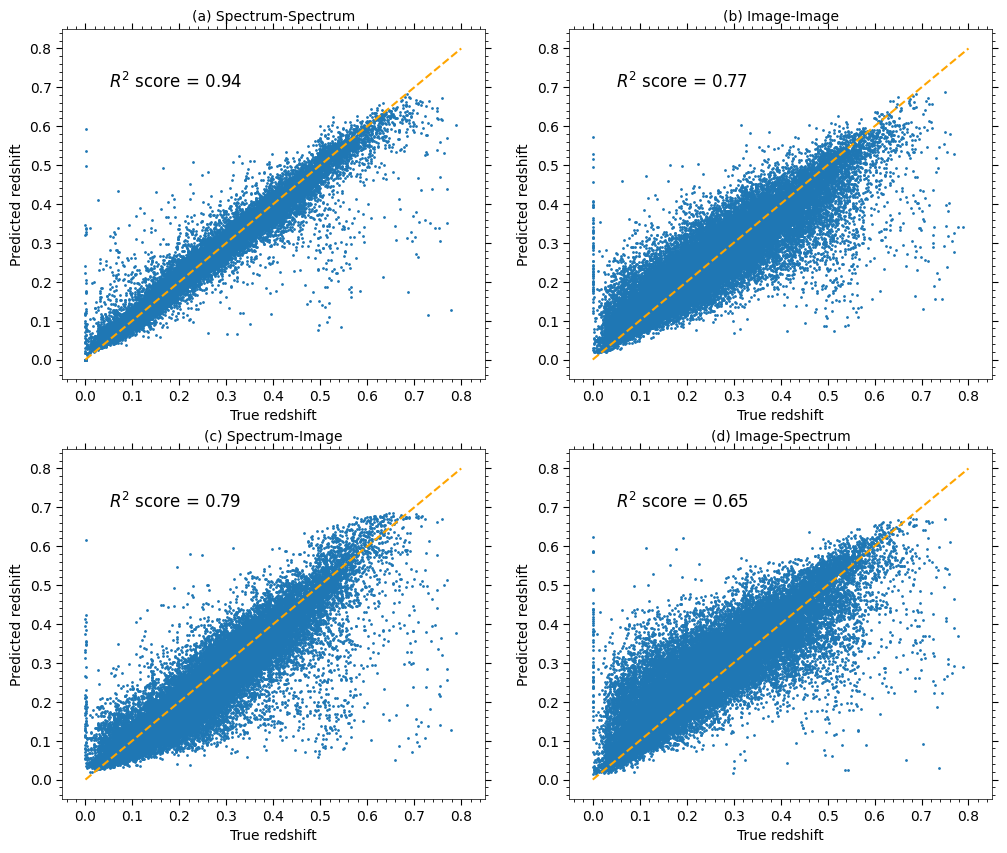
\includegraphics[width=1.2\textwidth]{figures/redshift_knn_regression}}
    \caption{In-modal and cross-modal zero-shot redshift predictions using k-NN regression on the learned embeddings. The y-axis shows
    the predicted redshift (the average of the 16 closest neighbours in terms of Euclidean distance) and the x-axis shows the true redshift.
    The dashed line represents a perfect prediction, and the $R^{2}$ of the fit is shown in the top left corner.
    $S_{kNN}(\mathbf{z}_{q}^{sp}, \mathbf{z}^{im})$ indicates the cross-modal prediction where a spectrums redshift was
    predicted using its 16 closes image embedded neighbours.}
    \label{fig:rkr}
\end{figure}

Figure~\eqref{fig:rkr} shows the zero-shot redshift predictions using k-NN regression on the learned embeddings for
both in-modal (spectrum to spectrum, image to image) and both cross-modal (spectrum to image, image to spectrum) predictions.
Both the spectrum-spectrum and image-image in-modal predictions fall slightly short of the predictive power of the
model trained by~\cite{astroclip} with our model achieving $R^{2}$ values of 0.94 and 0.74 respectively, compared to
0.79 and 0.98.
This is yields in interesting comparison on the effectiveness of the underlying architectures used, as well as pre-training
strategy.
The image and spectrum embedders utilised here were both CNNs and pre-trained as described in XXXXXXX, compared
to the transformer structure used in the original paper.
State-of-the-art galaxy spectra models thus far have traditionally been modelled using 1D convolutional architectures,
such as the one we have implemented in our AstroCLIP implementation.
A similar statement can be made on image embedders which have been traditionally modelled using 2D convolutional architectures.
However, these results indicate that the transformer architecture may be more effective in learning the underlying
representations of the data, as the original paper's model outperforms our implementation in both in-modal predictions.
Likewise, the pre-training performed by~\cite{astroclip} may have also been a more effective strategy for transfer learning
on this task XXXX WHAT IS THE PRE-TRAINING? WHAT METHODS WERE USED? XXXX.

\subsection{Retrieval by Cosine Similarity}\label{subsec:results-retrieval}
\begin{figure}[htb]
    \centering
    \makebox[\textwidth]{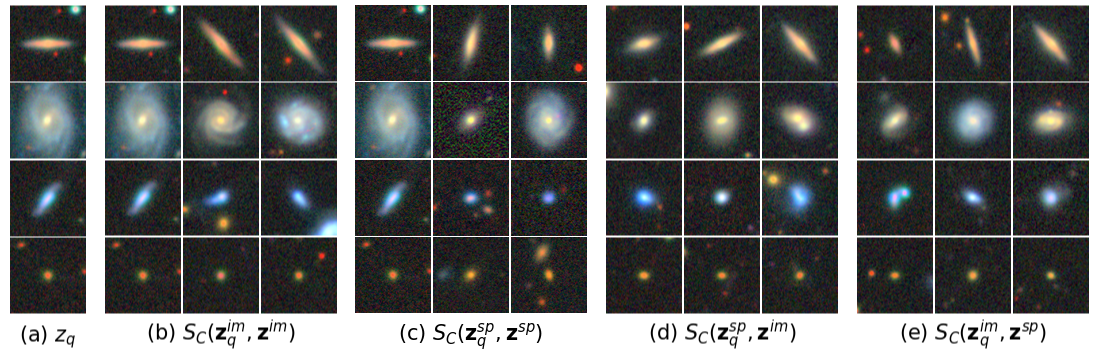
\includegraphics[width=1.2\textwidth]{figures/sim_search_images_all}}
    \caption{In-modal and cross-modal similarity search using cosine similarity on the learned embeddings.
        (a) shows the query galaxies; (b) shows the 3 most similar galaxies using an in-modal image to image search; and
        so on.
        By construction, the most similar in-modal galaxy to any given galaxy is itself, hence, the first column of images
        in (b) and (c) are identical to the query image in (a).}
    \label{fig:ssia}
\end{figure}

\begin{figure}[htb]
    \centering
    \makebox[\textwidth]{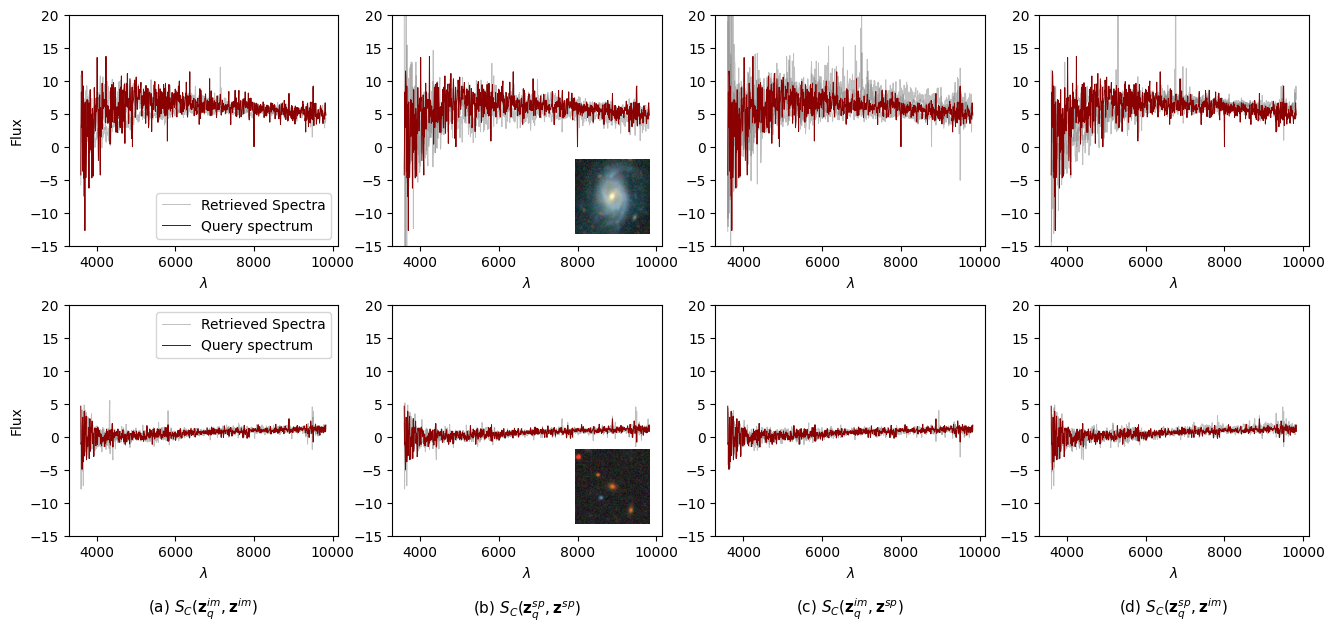
\includegraphics[width=1.2\textwidth]{figures/sim_search_spectra}}
    \caption{Similar to Figure~\eqref{fig:ssia}, each row in this figure depicts a single query galaxy (query spectrum in red,
        galaxy imaged in plot (b)), with each subfigure showing the spectrum of the 3 most cosine similar galaxies to the
        query galaxy by in-modal and cross-modal similarity search.}
    \label{fig:sss}
\end{figure}
